\section{Auswertung}
\label{sec:Auswertung}
\subsection{a) Effektiver Dämpfungswiderstand}
        Um den effektiven Dämpfungswiderstand zu bestimmen, werden die aufgenommenen Messwerte, der Spannung $U$ und der Zeit aus Tabelle 1, in der Form (\ref{eqn:e-spannung}) in ein Diagramm aufgetragen.
        \begin{figure}[H]
          \centering
          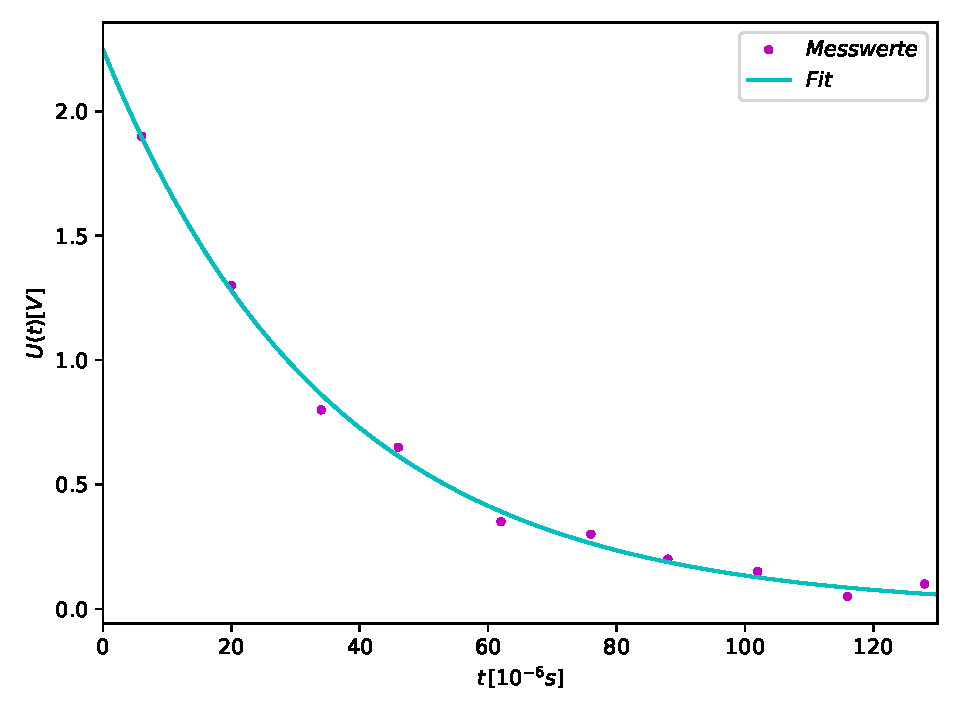
\includegraphics{a.pdf}
          \caption{Gemessene Spannung nach der Zeit aufgetragen}
        \end{figure}
        Mit $Python$ können dann die beiden unbekannten Größen $U_0$ und $2 \pi \cdot \mu$ von (\ref{eqn:e-spannung}) bestimmt werden, welche sich zu $U_0 = 2.25 V$ und $2\pi \cdot \mu = 0.03 \frac{\mathrm{V}}{\mathrm{H}}$ ergeben. Einsetzen in (\ref{eqn:R_eff}) liefert für den effektiven Dämpfungswiderstand
        \begin{equation*}
          R = 4 \pi \cdot \mu \cdot L = 98.7 \Omega \, .
        \end{equation*}
        Der Fehler berechnet sich mit (\ref{eqn:Fehlerfortpflanzung}) zu 
        \begin{equation}
            \increment R = \sqrt{\biggl(\frac{\partial R}{\partial L}\biggr)^2 \cdot (\increment L)^2} = 4 \pi \cdot \mu \cdot \increment L = 1.2 \cdot 10^{-12} \Omega,
        \end{equation}
        so dass sich für den effektiven Widerstand $R= 98.7 \pm 1.2 \cdot 10^{-12} \Omega$ ergibt.
        Die Abklingdauer $T_{ex}$ ist definiert als der Kehrwert von $2 \pi \cdot \mu$ definiert und berechnet sich mit (\ref{eqn:T_ex}) zu
        \begin{equation*}
          T_{ex} = \frac{1}{2\symup{\pi}\cdot \mu} = 0.01 s \, .
        \end{equation*}
\subsection{b) Dämpfungswiderstand beim aperiodischen Grenzfall}
        Im Versuch konnte der Widerstand $R_{ap} = 1.275 \, \symup{k\Omega}$ für den aperiodisichen Grenzfall abgelesen werden. Der theoretische Wert lässt sich mit (\ref{eqn:grenzwiderstand}) zu 
        \begin{equation*}
        R_{ap} = \sqrt{\frac{4L}{C}} = 1673.32\, \symup{\Omega}
        \end{equation*}
        berechnen. Was einer Abweichung von $23.8\%$ des gemessen Werts vom theoretischen Wert entspricht.
    \newpage
\subsection{c) Frequenzabhängigkeit der Kondensatorspannung}
        Die Frequenzabhängigkeit der Kondensatorspannung ist durch Gleichung (\ref{eqn:Kondensatorspannung.DGl}) gegben.
        Um die Kondensatorspannung in Abhänigigkeit der Frequenz zu bestimmen wurden Bereich $5-60$ kHZ die Kondensatorspannung bzw. die Spannung des Schwingkreises gemessen und in Tabelle 2 aufgetragen. Die Werte sind in Abbilgung 2 aufgetragen.
        \begin{figure}[H]
            \label{fig:Spannung}
             \includegraphics{Frequenzabhängigkeit.pdf}
            \caption{Kondensatorspannung in Abhänigigkeit der Frequenzabhängigkeit}
        \end{figure}
        Die Frequenzabhängigkeit der Kondensatorspannung ist durch Gleichung (\ref{eqn:spannung}) gegben. Mit den Werten $ L=3.5\cdot 10^{-3} \, \mathrm{H}$, $C=5.0 \cdot 10^{-9} \mathrm{F}$ und $R=271.6 \, \symup{\Omega}$ ergibt sich der Graph der Kondensatorspannung zu Abbildung 3.
        \begin{figure}[H]
            \label{fig:Spannung.theorie}
            \includegraphics{Frequenzabhängigkeit.theorie.pdf}
            \caption{Frequenzabhängigkeit der Kondensatorspannung in der Theorie}
        \end{figure}
        Es ist zu erkennen das die Kurve für die Kondensatorspannung die gemessen Werte in der Form annähert. Jedoch ist der Wert für die Resonanzfrequenz, in der Theorie deutlich höhere hat als die als die gemessene Resonanzfrequenz welche bei etwa $33 \, \symup{kHz}$ liegt. Während die theoretische Resonanzfrequenz sich mit (\ref{eqn:resonanz}) zu 
        \begin{equation*}
            \omega_{\symup{res}}= 232.66 \symup{kHZ}
        \end{equation*}
        ergibt. Was einer Abweichung von $85.82 \%$ von vom gemessen Wert zum theoretischen entspricht.
    \newpage
\subsection{d) Frequenzabhängigkeit der Phasenverschiebung}
        Nun soll Phase zwischen Erreger- und Kondensatorspannung in Abhänigigkeit von der Frequenz bestimmt werden.
        \begin{figure}[H]
            \label{fig:phase}
            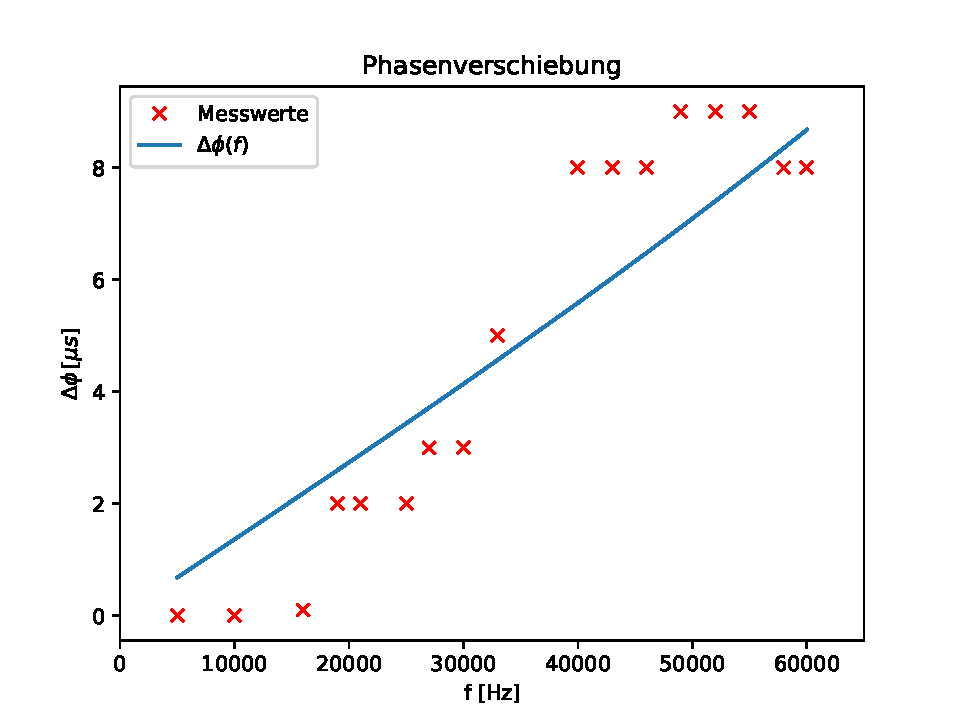
\includegraphics{Phasenverschiebung.pdf}
            \caption{Phasenverschiebung zwischen Erreger- und Kondensatorspannung}
        \end{figure}
        Die Phasenverschiebung lässt sich mit (\ref{eqn:phase}) bestimmen und ist in Abbildung 4 als die blaue Kurve dargestellt. (\ref{eqn:phase}) sagt aus, dass für hinreichend kleine Freqenzen die Kondensator- und Erregerspannung nahezu in Phase sind. Während bei höhereren Freqenzen die Kondensatorspannung ansteigt und am Höhepunkt etwa um $\pi$ hinter der Erregerspannung zurückbleibt. Dieses Verhalten des Anstiegs der Phasenverschiebung ist bei den Messwerten zu erkennen.
